\chapter{Introduction}
\label{ch1-intro} % a label for the chapter, to refer to it later

This is a book about \emph{combinatorial discrepancy theory} --- a
subject with roots in combinatorics, geometry, and number theory, and
numerous applications to other areas of mathematics and computer
science. In many of the applications, discrepancy provides a way to
``simplify'' a ``complex'' object. In this introductory chapter, we define the basic concepts in discrepancy theory, and illustrate the ways it can be applied with several examples.

\section{Discrepancy of Sets and Sparsification}

Consider the following balancing problem. We have a collection of subsets $\SS$ of some finite universe $\uni$, which we will call a \df{set system}. We want to color the universe $\uni$ with two colors, say red and blue, so that the red elements $R$, and the blue elements $B$ ``look similar'' to all the sets in $\SS$. I.e., each set in $\SS$ should have, as much as possible, a similar number of elements from $R$ and from $B$. Then the \df{discrepancy} of the coloring is 
\[
\max_{S \in \SS} \Big|\,|S\cap R| - |S \cap B|\,\Big|,
\]
and the discrepancy of the set system $\SS$ is the minimum discrepancy over all colorings, i.e., all partitions of $\uni$ into disjoint sets $R$ and $B$. It is convenient to encode a coloring as a function $\col:\uni \to \{-1,+1\}$,
% assigning $+1$ (corresponding to red) and $-1$ (corresponding to blue) values to $\uni$. 
where $\col(u)=+1$ corresponds to placing $u$ in $R$, and $\col(u)=-1$ corresponds to placing it in $B$. We further define $\col(S) \eqdef \sum_{\elem \in S}\col(\elem)$, which is just $|S\cap R| - |S \cap B|$.
We can now write the discrepancy of a coloring $\col$ and the discrepancy of $\SS$, respectively, as
\begin{align*}
    \disc(\SS,\col) &\eqdef \max_{S \in \SS}|\col(S)|,\\
    \disc(\SS) &\eqdef \min_{\col:\uni\to\{-1,+1\}} \disc(\SS,\col).
\end{align*}
Using Hoeffding's inequality, and the union bound, it is easy to see that, with probability at least $\frac12$, a uniformly random coloring $\col:\uni \to \{-1,+1\}$ achieves $\disc(\SS,\col) \lesssim \sqrt{|\uni|\log(2|\SS|)}$.\footnote{Here and in the
  rest of the book we use the notation $A\lesssim B$ to mean that
  $A \le CB$ for an absolute constant $C > 0$, and $A \gtrsim B$ to
  mean $B \lesssim A$.}  A major theme of this book, and of discrepancy theory in general, is the study of methods to construct colorings that achieve smaller discrepancy than random colorings. 

\paragraph{Application: Epsilon Approximations.} 
Most applications of the discrepancy of set systems rely on the observation that, because each set $S$ in $\SS$ is approximately equally split between the two color classes, restricting $S$ to one of the color classes reduces its size by approximately half. Thus, restricting all sets to the smaller color class gives another set system on a smaller universe, in which the relative sizes of the sets are preserved. 

Let us illustrate this idea with a geometric application. Let us take $P$ to be a finite point set in the plane. Let $\RR_2$ be the family of all axis-aligned rectangles, \ie, all sets of the
form $R = [a,b]\times [c,d]$. A subset $Q$ of $P$ is an $\varepsilon$-approximation of $P$ with respect to $\RR_2$, if for every axis-aligned rectangle $R$ we have that 
\[
\left|\frac{|Q \cap R|}{|Q|} - \frac{|P \cap R|}{|P|}\right| \le \varepsilon.
\]
I.e., $Q$ must be such that the fraction of points in it that land in any axis-aligned rectangle is equal, up to an additive error $\varepsilon$, to the fraction of points of $P$ that land in the same rectangle. Typically, we are interested in $\varepsilon$-approximations of small size. Such an $\varepsilon$-approximation is a concise approximation of the set system $\RR_2|_P \eqdef \{R\cap P: R \in \RR_2\}$ of subsets of $P$ induced by axis-aligned rectangles. Naturally, there is nothing special here about axis-aligned rectangles, and $\varepsilon$-approximations can be defined analogously for other families of geometric sets, e.g., halfspaces, or Euclidean balls, and in dimensions higher than 2. They are a useful concept in computational geometry. For example, a small $\varepsilon$-approximation immediately gives a small-space data structure for approximate range counting: the data structure is the $\varepsilon$-approximation $Q$, and given a query rectangle $R$, the number of points of $P$ in $R$ can be approximated by $|Q \cap R|\cdot |P|/|Q|$, which gives an additive approximation of $\varepsilon |P|$.


%Let us define $\disc(\RR_2,n)$ to be the maximum of $\disc(\RR_2|_P)$ over all $n$-point sets $P$. 
%The following lemma provides the connection between $\varepsilon$-approximations and discrepancy. 

%\begin{lemma}\label{lm:ch1-disc-epsapprox}
%    For any finite point set $P\subseteq \R^2$, there is a $\varepsilon$-approximation $Q$ of $P$ with respect to axis-aligned rectangles
%\end{lemma}

Discrepancy gives us a way to construct an $\varepsilon$-approximation $Q$ of half the size of $P$. Let us denote $n\eqdef |P|$. Suppose that, for the set system $\SS \eqdef \RR_2|_P$ induced by axis-aligned rectangles on $P$, the coloring $\col$ achieves $D \eqdef \disc(\SS)$, and let $Q$ be the points in $P$ colored $+1$. The discrepancy constraint implies that for every rectangle $R \in \RR_2$,
\[
\Big||Q\cap R| - |(P\setminus Q) \cap R|\Big| \le D.
\]
On the other hand, $|P\cap R| = |Q\cap R| + |(P\setminus Q) \cap R|$, so
\[
\Big||Q\cap R| - \frac12 |P \cap R|\Big|
= 
\frac12 \Big||Q\cap R| - |(P\setminus Q) \cap R|\Big| \le \frac{D}{2}.
\]
If the size of $Q$ were exactly $n/2$, then dividing both sides by $|Q|$ would give us that $Q$ is a $D/n$-approximation to $P$ with respect to axis-aligned rectangles. But now we can observe that some axis-aligned rectangle contains all the points in $P$, so the discrepancy bound also implies that $\left||Q| -  n/2\right| \le D/2$. Then, we can make sure that $|Q| = n/2$ by adding or removing at most $D/2$ points from it, and this modified $Q$ is a $2D/n$-approximation. 

Let $\disc(\RR_2,n)$ be the maximum of $\disc(\RR_2|_P)$ over all $n$-point sets $P$. The argument above gives us the following lemma.

\begin{lemma}\label{lm:ch1-disc-epsapprox}
    For any $n$-point set $P\subseteq \R^2$, there is an $\varepsilon$-approximation $Q$ of $P$ with respect to axis-aligned rectangles such that $|Q| = n/2$ and $\varepsilon\le 2\disc(\RR_2,n)/n$.
\end{lemma}

We will see later in Chapter~\ref{ch:gamma2} that $\disc(\RR_2, n) \lesssim \log^{1.5}(2n)$.
Thus the $\varepsilon$ in Lemma~\ref{lm:ch1-disc-epsapprox} is very close to $0$ when $n$ is large. Typically, however, we can settle for a constant $\varepsilon$, but would like $|Q|$ to only depend on $\varepsilon$. We can achieve this by applying Lemma~\ref{lm:ch1-disc-epsapprox} repeatedly, together with the following simple composition lemma, whose proof is left as an exercise.

\begin{lemma}\label{lm:ch1-epsapprox-composition}
    If $Q_1$ is an $\varepsilon_1$-approximation of $P$, and also $Q_2$ is an $\varepsilon_2$-approximation of $Q_1$, then $Q_2$ is an $(\varepsilon_1 + \varepsilon_2)$-approximation of $P$.
\end{lemma}

We can now apply Lemma~\ref{lm:ch1-disc-epsapprox} repeatedly, each time halving the size of $Q$, and Lemma~\ref{lm:ch1-epsapprox-composition} tells us that the approximations add up. If we stop at a set $Q$ of $s$ points, we have that $Q$ is an $\varepsilon$-approximation for 
\[
\varepsilon = \frac{2 \disc(\RR_2, n)}{n} + \frac{4 \disc(\RR_2, n/2)}{n} + \ldots + \frac{\disc(\RR_2, 2s)}{s}\lesssim \frac{\disc(\RR_2, n)}{s},
\]
where the last bound follows since $\disc(\RR_2, n)$ grows polylogarithmically in $n$. Plugging in $\disc(\RR_2, n) \lesssim \log^{1.5}(2n)$ and solving for $s$, we get the following theorem.

\begin{theorem}\label{thm:ch1-rectangles}
     For any $\varepsilon \in (0,1)$, and any $n$-point set $P\subseteq \R^2$, there is an $\varepsilon$-approximation $Q$ of $P$ with respect to axis-aligned rectangles such that $|Q| \lesssim (\log^{1.5}(1/\varepsilon))/\varepsilon$.
\end{theorem}

Note that, as long as we can efficiently find a coloring $\col$ of any $n$ points $P$ achieving $\disc(\RR_2|_P,\col) \lesssim \log^{1.5}(2n)$, we can also perform the construction in Theorem~\ref{thm:ch1-rectangles} efficiently. Unfortunately, no such efficient algorithm is known for this bound, but the slightly weaker bound $\disc(\RR_2|_P,\col) \lesssim \log^{2}(2n)$ can be achieved in polynomial time using the methods of Chapter~\ref{ch:algo-komlos-bana}.

The size bound in Theorem~\ref{thm:ch1-rectangles} would be immediately improved by improving the bound on the discrepancy $\disc(\RR_2,n)$. This motivates the following problem, to which we return several times in this book.

\begin{problem}\label{prob:tusnady}
  Determine the maximum discrepancy of a set system induced by the family $\RR_d$ of
  \(d\)-dimensional axis-aligned boxes (cross
products of $d$ intervals) on an \(n\)-point set, \ie,
  give tight bounds on 
  \(
    \disc(\RR_d, n) \eqdef \max\{\disc(\RR_d|_P): P \subseteq \R^d, |P| = n\}.
  \)
\end{problem}
Later in the book we will see upper and lower bounds on $\disc(\RR_d, n)$ that are tight within a $O(\sqrt{\log n})$ factor.

Bounds on $\varepsilon$-approximations with respect to other families of geometric sets similar to Theorem~\ref{thm:ch1-rectangles} can be proved using the same argument and bounds on the discrepancy of the appropriate set system. 

\section{Discrepancy of Matrices and Rounding}

The discrepancy of a set system can be written in a linear algebraic way, which also suggests a natural way to define discrepancy of a matrix. Let $\SS$ be a set system on a universe $\uni$, and let us take
$\mat$ to be the incidence matrix of $\SS$,
\ie, the matrix with rows indexed by $\SS$, columns indexed by $\uni$, and entries equal to 
\[
  \mat(S,\elem) \eqdef
  \begin{cases}
    1 & \text{if } \elem \in S\\
    0 &  \text{if } \elem \not \in S
  \end{cases}
\]
for any $S \in \SS$ and $\elem \in \uni$.\footnote{We identify $n$-dimensional vectors $x$ with functions $x:[n] \to \R$, where $x(i)$ is the $i$-th coordinate of $x$, and $m\times n$ matrices $M$ with functions $M:[m]\times [n] \to \R$, where $M(i,j)$ is the entry in row $i$ column $j$ of $M$.} Then it is easy to check that 
\begin{align*}
\disc(\SS,\col) &= \max_{S \in \SS} |(\mat\col)_S| = \|\mat \col\|_{\infty},\\
\disc(\SS) &= \min_{x \in \{-1,1\}^\uni} \|\mat\col\|_\infty.
\end{align*}
Inspired by these observations, we can then define the discrepancy of any $m\times n$ matrix $\mat$ and a coloring $\col \in \{-1,+1\}^n$ as $\disc(\mat,\col) \eqdef \|\mat\col\|_\infty$, and the discrepancy of the matrix $\mat$ as $\disc(\mat) \eqdef \min_{\col \in \{-1,+1\}^n} \|\mat\col\|_\infty$.

\paragraph{Application: Rounding}
Suppose that $y \in [0,1]^n$ satisfies the constraints $\mat y = b$ for some $m\times n$ matrix $\mat$ and $m$-dimensional vector $b$. For example, $y$ can be the solution to a linear programming relaxation of a combinatorial optimization problem. Matrix discrepancy allows us to round $y$ to a binary vector $z \in \{0,1\}^n$ so that the constraints are approximately satisfied. 

The simplest case is rounding a vector $y$ all of whose coordinates are equal to $\frac12$, i.e., $y = \frac12 \ones$, where $\ones$ is the all-ones vector. Then, if $\col \in \{-1,+1\}^n$ achieves $\|\mat \col\|_\infty = \disc(\mat)$, for the binary vector $z \eqdef  y + \frac12\col$ we have
\[
\left\|\mat z - b\right\|_\infty = \|\mat(z-y)\|_\infty
= 
\frac12 \|\mat \col\|_\infty = \frac{\disc(\mat)}{2}.
\]
This is, in fact, essentially the same observation as the one used in Lemma~\ref{lm:ch1-disc-epsapprox}. If $y$ is instead half-integral, i.e., its coordinates are in $\left\{0,\frac12, 1\right\}$, then we can apply the same construction, but only to the coordinates equal to $\frac12$. The resulting error in our rounding will be half the discrepancy of the submatrix of $\mat$ corresponding to these coordinates. In general, to round arbitrary vectors $y$ using this method, we need a bound on the maximum discrepancy of any submatrix of $\mat$. This motivates the definition of \df{hereditary discrepancy}:
\[
\herdisc(\mat) \eqdef \max_{J \subseteq [n]}\disc(\mat(*,J)),
\]
where $\mat(*,J)$ is the submatrix of $\mat$ consisting of the columns indexed by $J$. By applying the idea above to the bit representation of $y$, we get the following rounding result. 

\begin{theorem}\label{thm:ch1-transference}
  For any $m\times n$ matrix $\mat$,
  and any $y \in [0,1]^n$,
  there exists some $z \in \{0,1\}^n$ such that 
  \[
    \left\|\mat (z-y)\right\|_\infty
    \le
    \herdisc(\mat).
  \]
  % Moreover, we have the bound
  % \[
  %   \left\|\sum_{i = 1}^n (x_i - y_i) u_i\right\|_X
  %   \le
  %   \sum_{k = 1}^\infty 2^{-k}\herdisc_X\left((u_i)_{i = 1}^n, 2^{k}\sum_{i = 1}^n y_i\right).
  % \]
\end{theorem}
\begin{proof}
  Let us assume that there is some finite $k$ such that, for each $j \in [n]$, $y(j) \in 2^{-k} \mathbb{Z}$, \ie, that each coordinate $y(j)$
  can be written using at most $k$ bits after the radix point. By standard compactness arguments, it is
  enough to show that the theorem holds under this assumption. Suppose that, for every $j$,
  $b_k(j)$ is the $k$-th bit after the radix point of $y(j)$, and $y'(j)$ is the real number given by the first $k-1$ bits after the radix point. Then $y(j) = y'(j) + 2^{-k} b_k(j)$. Let $J = \{j: b_k(j) = 1\}$, and find a
  coloring $\col\in \{-1,+1\}^J$ which achieves
  \[
  \|\mat(*,J) \col\|_\infty = \disc(\mat(*,J)) \le \herdisc(\mat).
  \]
  We set, for all $j \in J$,
  \[
    y''(j) \eqdef  y(j) + \col(j)2^{-k} = y'(j) + 2^{-k} + \col(j)2^{-k},
  \]
  and $y''(j) \eqdef y'(j) = y(j)$ for $j \not \in J$. I.e., for every coordinate $y(j)$ whose $k$-th bit after the radix point is $1$, we round that bit up if $x(j) = +1$, or down otherwise.
  Clearly each 
  \(
  y''(j)
  \)
  can be written with at most $k-1$ bits after the radix point,
  and
  \[
  \|\mat (y''-y)\|_\infty = 2^{-k}\|\mat(*,J)\col\|_\infty\le 2^{-k}\herdisc(\mat).
  \]
  We then replace $y$ with $y''$ and $k$ with $k-1$, and inductively apply the same bit-rounding process until $k = 0$, at which point we have our vector $z \in \{0,1\}^n$. Summing the errors from rounding each bit, we get 
  \[
  \|\mat (z-y)\|_\infty \le (2^{-1} + 2^{-2} + \ldots + 2^{-k})\herdisc(\mat) \le \herdisc(\mat). \qedhere
  \]
\end{proof}

Theorem~\ref{thm:ch1-transference} can be used to derive a result similar to Theorem~\ref{thm:ch1-rectangles}. We let $\mat$ be the incidence matrix of $\RR_2|_P$, and $y = \frac{s}{n}\ones$. Applying Theorem~\ref{thm:ch1-transference} and letting $Q\eqdef \{p \in P:z(p) = 1\}$, we have that, for any rectangle $R \in \RR_2$,
\[
\left||Q\cap R| - \frac{n}{s}|P\cap R|\right| \le \herdisc(\RR_2|_P) \le \disc(\RR_2,n) \lesssim \log^{1.5}(2n).
\]
Moreover, since some rectangle contains all of $P$, we also have $||Q| - s| \lesssim \log^{1.5}(2n)$, so up to a constant factor increase in the bound above, we can assume that $|Q| = s$. Thus, dividing the inequality above by $s$ gives us that $Q$ is an $(\log^{1.5}n)/s$-approximation. Unfortunately, this is not quite enough to get the bound in Theorem~\ref{thm:ch1-rectangles} or any bound that depends entirely on $\varepsilon$. We can address this with a slight strengthening of Theorem~\ref{thm:ch1-transference}. Let us define a parametrized version of hereditary discrepancy by 
\[
\herdisc(\mat,s) \eqdef \max_{J\subseteq [n]: |J| \le s}\disc(\mat(*,J)).
\]
We then have the stronger rounding result stated next, which follows by essentially the same proof.
\begin{theorem}\label{thm:ch1-transference-sizes}
For any $m\times n$ matrix $\mat$, and any $y \in [0,1]^n$, there exists some $z \in \{0,1\}^n$ such that 
\[
    \left\|\mat(z-y)\right\|_\infty
    \le
    \sum_{k = 1}^\infty 2^{-k}\herdisc\left(\mat, 2^{k}\sum_{j = 1}^n y_j\right).
\]
\end{theorem}
\begin{proof}
    We construct $z$ in the same way as in Theorem~\ref{thm:ch1-transference}, and simply observe that the set $J = \{j: b_k(j) = 1\}$ of coordinates of $y$ with $k$-th bit after the radix point equal to $1$ is of size at most $2^k\sum_{j = 1}^n y_j$. 
\end{proof}
Theorem~\ref{thm:ch1-transference-sizes} now allows us to recover Theorem~\ref{thm:ch1-rectangles} since $\herdisc(\RR_2|_P,s) \le \disc(\RR_2,s) \lesssim \log^{1.5}(2s)$. 

Moreover, as with Theorem~\ref{thm:ch1-rectangles}, the roundings in Theorems~\ref{thm:ch1-transference}~and~\ref{thm:ch1-transference-sizes} can found efficiently as long as we can find colorings with discrepancy bounded by the hereditary discrepancy. We return to this question in Chapter~\ref{ch:partial-alg}. 

\section{Vector Balancing and Approximate Carath\'eodory}

While the infinity norm is natural for the discrepancy of set systems, and for measuring how much a rounded solution to a system of linear equations violates the equations, in other applications of matrix discrepancy we may need to consider other norms. The definitions we made above can be generalized easily to such a setting. Suppose $\|\cdot\|_X$ is some norm on $\R^m$, and let $X$ be the corresponding normed space. Then, the discrepancy of a coloring $\col \in \{-1,+1\}^n$ with respect to an $m\times n$ matrix $\mat$ and $X$ is $\disc_X(\mat,\col) \eqdef \|\mat \col\|_X$. The discrepancy of $\mat$ with respect to $X$ is $\disc_X(\mat) \eqdef \min_{\col \in \{-1,+1\}^n} \|\mat\col\|_X$. Hereditary discrepancy is again defined by taking a maximum over submatrices:
\begin{align*}
    \herdisc_X(\mat,s) &\eqdef \max_{J\subseteq [n]: |J| \le s}\disc_X(\mat(*,J)),\\
    \herdisc_X(\mat) &\eqdef \max_{J\subseteq [n]}\disc_X(\mat(*,J)).
\end{align*}
It is easy to check that, since the proofs only use the triangle inequality and homogeneity properties of the $\ell_\infty$ norm, Theorems~\ref{thm:ch1-transference}~and~\ref{thm:ch1-transference-sizes} hold under any norm. Next we consider the $\ell_2$ norm, and give another geometric application of these rounding theorems.

\paragraph{Approximate Carath\'eodory Theorem.} Let $u_0, u_1, \ldots,
u_n$ be vectors in  $\R^m$, and let $v$ be a point in their convex hull. Carath\'eodory's theorem shows that there exists a subset $S
\subseteq \{0\} \cup [n]$ of cardinality at most $m+1$ so that $v$ is
also in the convex hull of $\{u_i: i \in S\}$. This is generally
tight, for example when $u_0 = 0$, $u_i$ is the $i$-th standard basis
vector of $\R^m$, and $v$ is the vector with every coordinate equal to
$\frac{1}{m+1}$. However, if we only ask $v$ to be \emph{close} to the
convex hull of $\{u_i: i \in S\}$, then perhaps we can hope to improve the
bound on the size of $S$, and, moreover, we can hope for bounds
that are independent of the dimension $m$.

Once we allow for approximation, we need to fix a way to measure distances, and a scale. We will, for now, pick the Euclidean, i.e., $\ell_2$ distance. As for fixing a scale, a
natural way to do so is to ask that the diameter
\(
\max_{i = 0}^n\max_{j = 0}^n\|u_i - u_j\|_2
\)
be bounded by $1$. 
Since everything in our set up is invariant under translation, we can
assume that $u_0 = 0$, and, by the diameter condition, $\|u_i\|_2 \le
1$ for all $i \in[n]$.

We will use discrepancy to approximate $v$ by the average of $s$ vectors, for a parameter $s$, so that the approximation error scales like $\min\left\{\frac{\sqrt{m}}{s}, \frac{1}{\sqrt{s}}\right\}$.
To this end, let us explicitly write $v$ as a convex combination of $u_0, \ldots u_n$ as
\begin{align*}
    v = \alpha_0 u_0 + \alpha_1 u_1 + \ldots + \alpha_n u_n
    = \alpha_1 u_1 + \ldots + \alpha_n u_n
\end{align*}
for some $\alpha_1, \ldots, \alpha_n \ge 0$ such that $\sum_{i=1}^n \alpha_i \le 1$. By Carath\'eodory's theorem we can assume that $n \le m$. Inspired by the proof of Theorem~\ref{thm:ch1-rectangles} via Theorem~\ref{thm:ch1-transference}, let us define $y \in \R^n$ by $y(i) \eqdef s \alpha_i$. Take $z \in \{0,1\}^n$ to be the rounding of $y$ guaranteed by Theorem~\ref{thm:ch1-transference} when used with the $\ell_2$ norm and the matrix $\mat$ with columns $u_1, \ldots, u_n$. Let $S \eqdef \{i: z(i) = 1\}$.\footnote{Technically, we use Theorem~\ref{thm:ch1-transference} to round the vector with coordinates $y(i) - \lfloor y(i)\rfloor$, and we first add $\lfloor y(i) \rfloor$ copies of $i$ to $S$ before adding also those $i$ for which $z(i) = 1$.} We then have that
\begin{equation}\label{eq:ch1-apxcar-rounding}
   \left\|sv - \sum_{i\in S} u_i\right\|_2 \le \herdisc_{\ell_2}(\mat). 
\end{equation}
Moreover,  for a uniformly random $\col \in \{-1,+1\}^n$, and a matrix $\mat$ with $n$ columns each of $\ell_2$ norm at most $1$, $\E \|\mat\col\|_2^2 \le n$. Therefore, $\disc_{\ell_2}(\mat) \le \sqrt{n}$, and, since this reasoning applies to any submatrix as well, $\herdisc_{\ell_2}(\mat) \le \sqrt{n}$. We have 
$
\left\|sv - \sum_{i\in S} u_i\right\|_2 \le \sqrt{n}\le \sqrt{m}.$

If we could guarantee that $|S| = s$, then dividing both sides of the inequality by $s$ would guarantee that 
\[
\left\|v - \frac{1}{|S|}\sum_{i\in S} u_i\right\|_2 \le \frac{\sqrt{m}}{s}.
\]
Unfortunately, we cannot automatically deduce that $|S|$ is close to $s$ from~\eqref{eq:ch1-apxcar-rounding}. Nevertheless, there is a simple workaround, given in the following corollary of Theorems~\ref{thm:ch1-transference}~and~\ref{thm:ch1-transference-sizes}.
\begin{corollary}\label{cor:ch1-transference}
    In both Theorem~\ref{thm:ch1-transference} and Theorem~\ref{thm:ch1-transference-sizes}, we can assume that $\sum_{j=1}^n z(j) \le \sum_{j=1}^n y(j)$.
\end{corollary}
\begin{proof}
    Follows from the same proof we gave for the theorems, after noticing that we can always take the coloring $\col \in \{-1,+1\}^J$ to be such that $\sum_{j \in J}\col(j) \le 0$ since if this is not the case, we can just flip the colors without changing the discrepancy.
\end{proof}

We can now show the following result.
\begin{theorem}\label{thm:ch1-apxcarath-L2}
    Suppose that $u_0, \ldots, u_n$ are vectors in $\R^m$, and their diameter is at most $1$. For any vector $v$ in their convex hull, and any positive integer $s$, there exists a (multi-)set $S \subseteq \{0\} \cup [n]$ of size $s$ such that 
    \[
    \left\|v - \frac{1}{s} \sum_{i \in S} u_i\right\|_2 \lesssim \min\left\{\frac{\sqrt{m}}{s}, \frac{1}{\sqrt{s}}\right\}.
    \]
\end{theorem}
\begin{proof}
    As above, we may assume $n \le m$, shift the vectors so that $u_0 = 0$, and write $v = \alpha_1 u_1 + \ldots + \alpha_n u_n$ for non-negative $\alpha_1, \ldots, \alpha_n$ that sum to at most $1$. Define $y \in \R^n$ by $y(i) \eqdef s \alpha_i$. If some $y(i)$ is larger than $1$, then we add $\lfloor y(i)\rfloor$ copies of $i$ to $S$, and replace $y(i)$ by $y(i) - \lfloor y(i)\rfloor$. We can now apply Corollary~\ref{cor:ch1-transference} to $y$ to get a vector $z \in \{0,1\}^n$, and add all $i$ such that $z(i) = 1$ to $S$. By the guarantee of the corollary, we have that $|S| \le s\sum_{i=1}^n\alpha_i = s$. To make sure $S$ has size exactly $s$, we add sufficiently many copies of $0$ to $S$. 
    
    Recall the observation above that $\disc_{\ell_2}(\mat,\col) \le \sqrt{n}$ for an $n$-column matrix $\mat$ with columns whose $\ell_2$ norms are at most $1$. Therefore $\herdisc(\mat,t) \le \sqrt{t}$ for such a matrix, and the theorem follows from the inequality \eqref{eq:ch1-apxcar-rounding} and the more precise bound
    \[
    \left\|sv - \sum_{i\in S} u_i\right\|_2 \le \sum_{k=1}^\infty 2^{-k}\herdisc_{\ell_2}(\mat,2^ks)
    \lesssim \sqrt{s}\sum_{k=1}^\infty 2^{-k/2}\lesssim \sqrt{s}.
    \qedhere \]
\end{proof}

The key quantity in the proof of Theorem~\ref{thm:ch1-apxcarath-L2} is a vector balancing constant. Suppose $K$ is some subset of $\R^m$, and $\|\cdot\|_X$ is, as above, a norm on $\R^m$. The vector balancing constants for $K$ and $X$ are defined by
\begin{align*}
  \vb(K,X,n) &\eqdef \sup\{\disc_X((u_i)_{i=1}^n): u_1, \ldots, u_n  \in K\},\\
  \vb(K,X) &\eqdef \sup_n \vb(K,X,n). 
\end{align*}
In our proof of Theorem~\ref{thm:ch1-apxcarath-L2} we used the simple observation that $\vb(B_{\ell_2},\ell_2,n) \le\sqrt{n}$, where $B_{\ell_2} \eqdef \{u: \|u\|_2 \le 1\}$ is the unit ball. The same proof shows that if the vectors $u_0, \ldots, u_n$ have diameter bounded by $1$ in the norm $\|\cdot\|_X$, then we can guarantee
\[
    \left\|v - \frac{1}{|S|} \sum_{i \in S} u_i\right\|_X \le
    \frac{1}{s} \sum_{k = 1}^\infty 2^{-k}\vb(B_X, X, 2^{k}s),
\]
where $B_X \eqdef \{u \in \R^m: \|u\|_X \le 1\}$.

There is also no reason why
the diameter of $u_0, \ldots u_n$ has to be bounded in the same norm in
which we measure the approximation. For example, in the next chapter,
we will see that $\vb(B_{\ell_1},\ell_\infty) \le 2$ (this is a
result of Beck and Fiala~\cite{BF81}). Then, using analogous reasoning to the above, we have that whenever $u_0, \ldots,
u_n$ have $\ell_1$ diameter at most $1$, for any point $v$ in their
convex hull we can find an average $v'$ of $s$ vectors from
$u_0, \ldots, u_n$ so that $\|v - v'\|_\infty \le
\frac{2}{s}$. Remarkably, it is an open problem whether this 
$\|v - v'\|_\infty \lesssim \frac{1}{s}$
error bound can be achieved under the weaker assumption that $u_0, \ldots,
u_n$ have Euclidean diameter at most $1$. Such an improvement would
follow from a positive solution to the following problem, due to
Koml\'os. 
\begin{problem}\label{prob:komlos}
  Prove or disprove the bound $\vb(B_{\ell_2^m},\ell_\infty^m)
  \lesssim 1$.
\end{problem}

Later in the book, we will see partial progress towards
Problem~\ref{prob:komlos}, and, in particular, a bound of
$O(\sqrt{\log m})$ due to Banaszczyk~\cite{Bana98}. We will see both
Banaszczyk's result in Chapters \ref{ch:bana-intro} and \ref{ch:bana-proof}, and also two different proofs in Chapter \ref{ch:algo-komlos-bana} and \ref{ch:gram-schmidt} that gives an efficient
algorithm to construct the coloring achieving this bound.\footnote{Very recently, Bansal and Jiang \cite{bansaljiang2025} have obtained an $O(\log^{1/4} m)$ discrepancy bound for the Koml\'{o}s problem, building on the techniques we will see in Chapter \ref{ch:algo-komlos-bana}. However, we will not discuss their result in this book.}


\section{Prefix Discrepancy and the Steinitz Problem}
\label{sec:ch1-steinitz}

Suppose an $m\times n$ matrix $\mat$ has columns $u_1, \ldots, u_n \in \R^m$. A useful strengthening of matrix discrepancy is prefix discrepancy, which requires that the same coloring simultaneously balances each prefix of columns $u_1, \ldots, u_i$. Formally, we define the \df{prefix discrepancy} of a matrix $\mat$ with columns $u_1, \ldots, u_n$, and a coloring $\col \in \{-1,+1\}^n$   as 
\[
\pdisc(\mat, \col) \eqdef
\max_{j=1}^n \left\|\sum_{i = 1}^j\col(i)u_i \right\|_\infty.
\]
The prefix discrepancy of $\mat$ is the minimum of $\pdisc(\mat, \col)$ over all colorings $\col \in \{-1,+1\}^n$. Similarly to matrix discrepancy, we can also define a variant $\pdisc_X(\mat)$ in which the $\ell_\infty$ norm is replaced by some other norm $\|\cdot\|_X$ on $\R^m$.

This is a natural generalization of discrepancy when we decide on the colors $\col(1), \ldots, \col(n)$ one at a time, e.g., because the column vectors $u_1, \ldots, u_n$ are specified online. We will also see that prefix discrepancy can be used to prove bounds on standard discrepancy in problems with some implicit ordering: this will be the approach we take for Problem~\ref{prob:tusnady} in Chapter~\ref{ch:gamma2}. Here we will see another application to a classical geometric problem. 

\paragraph{The Steinitz Problem.} Suppose we have vectors $u_1, \ldots, u_n$ in $\R^m$, so that each vector is ``short'',
\ie, $u_i \in [-1,+1]^m$ for all $i$. If
$u_1 + \ldots + u_n = 0$, then the partial sums $u_1 + \ldots + u_j$
trace a path in space from the origin back to itself. At intermediate
steps, the path can be arbitrarily far from $0$, but it always takes
short steps. Can we re-arrange the vectors, so that the path always
stays close to $0$, and, in particular, the norm
\( \left\|\sum_{i = 1}^j u_i\right\|_\infty\) of each partial sum is
always bounded by a function depending only on the dimension $m$? See
Figure~\ref{fig:ch1-steinitz} for an illustration.

\begin{figure}[htp]
  \centering
  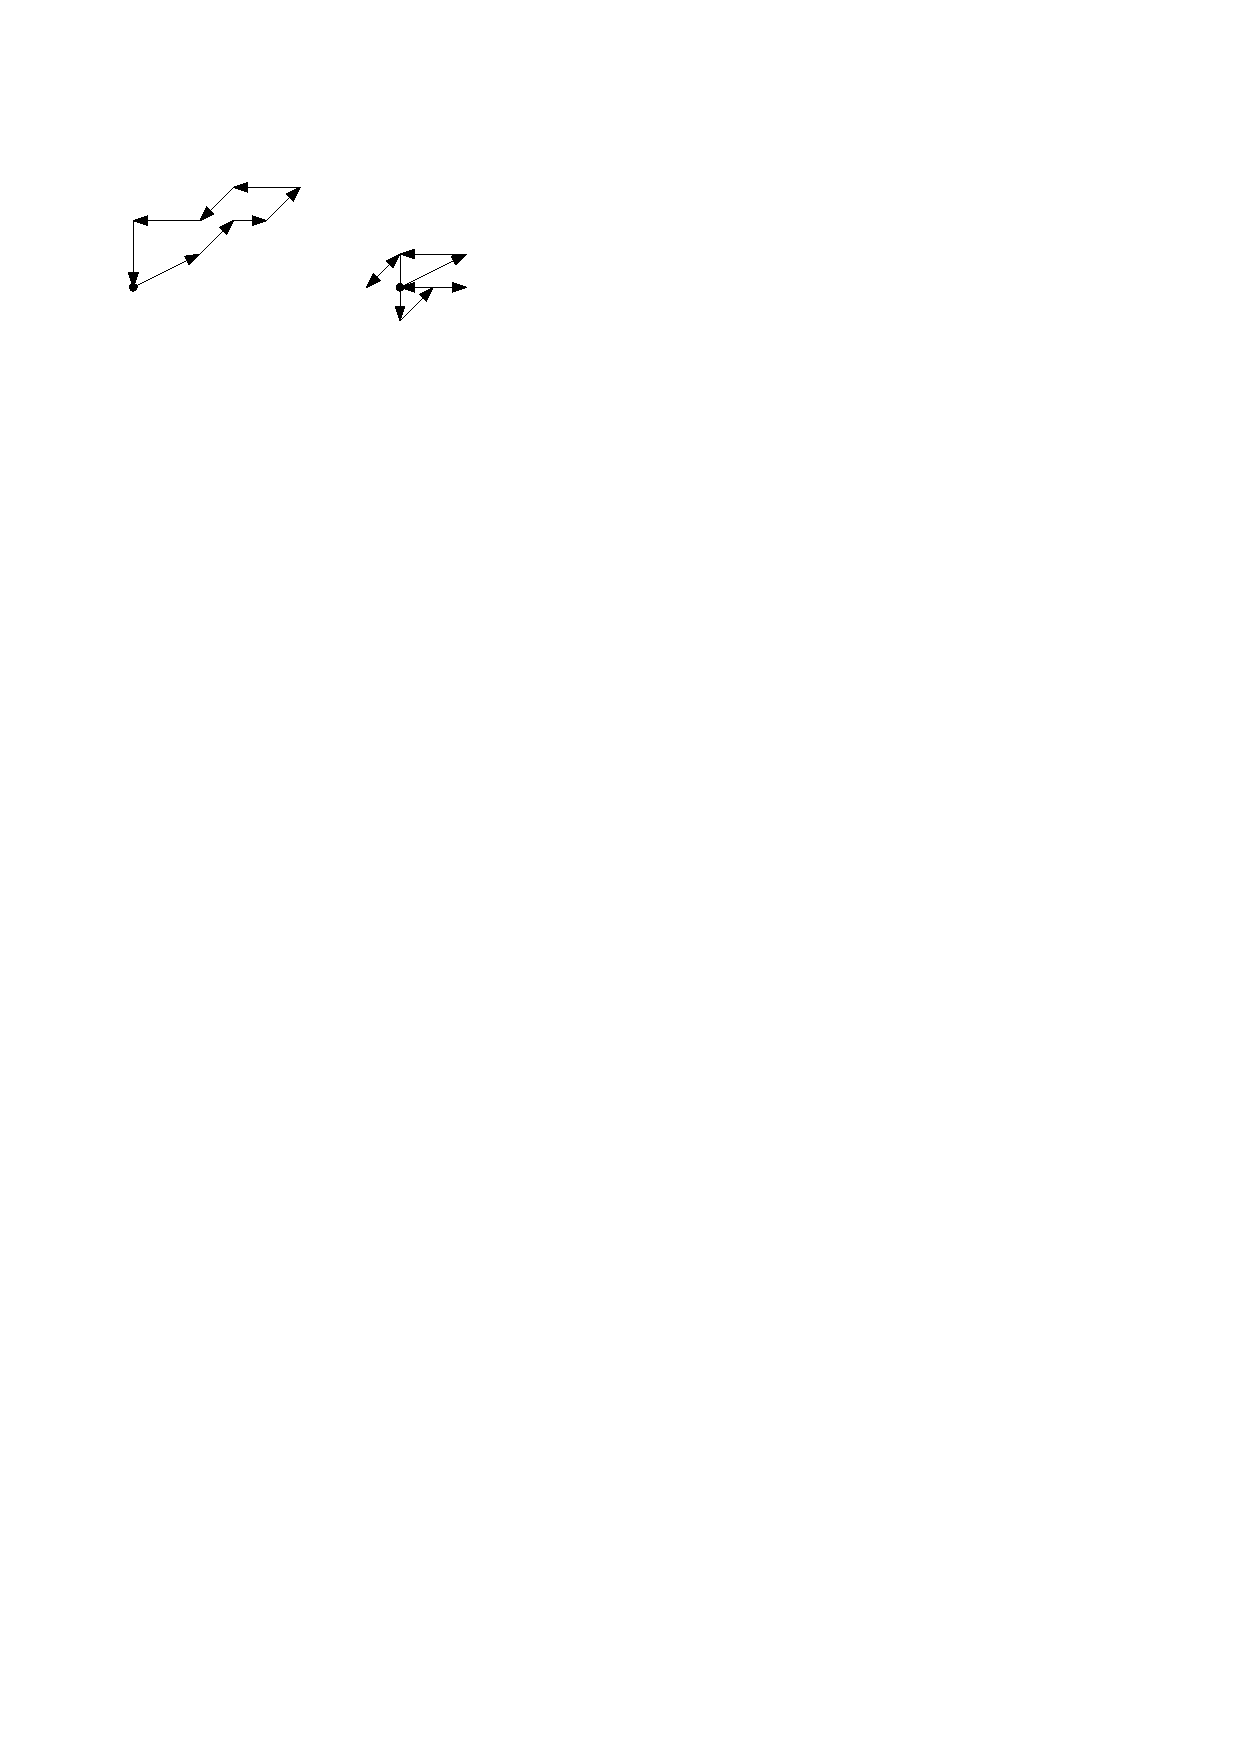
\includegraphics{steinitz}
  \caption[Rearrangement of a path]{A path of short steps returning to
    the origin, and a rearrangement of the steps so that the path
    stays much closer to the origin.}
  \label{fig:ch1-steinitz}
\end{figure}

This question was first asked (and answered affirmatively) by
Steinitz~\cite{Steinitz1913}. Note that the requirement that the vectors
sum to $0$ is not essential. In general, if $v = u_1 + \cdots + u_n$
is the sum of the vectors; then we can make sure that the path
traced by the partial sums stays close to the line from $0$ to $v$,
\ie, that
\(
\left\|\frac{j}{n}v - \sum_{i = 1}^j u_i\right\|_\infty  
\)
is as small as possible for all $j \in [n]$. This question is, however, essentially equivalent to the version where the vectors sum to $0$, which we can see by replacing each $u_i$ with $u_i - \frac{1}{n}v$. 

The Steinitz problem arises
naturally in many contexts, e.g.~in designing algorithms for integer
programming~\cite{EisenbrandW20}, and approximation algorithms for
scheduling problems~\cite{Sev78}. Let us use the notation $\st((u_i)_{i=1}^n)$ for how close we can keep the path to the line from $0$ to $v$, i.e., 
\[
\st((u_i)_{i=1}^n) \eqdef \min_{\pi \in S_n} \max_{j=1}^n \Bigg\|\frac{j}{n} v - \sum_{i=1}^j u_{\pi(i)}\Bigg\|_\infty,
\]
where $S_n$ is the set of permutations of $[n]$, and $v \eqdef \sum_{i = 1}^n u_i$. Once again, this question also makes sense for any norm $\|\cdot\|_X$ in place of the $\ell_\infty$ norm, and we denote the corresponding quantity by $\st_X((u_i)_{i=1}^n)$.

Prefix discrepancy is a very useful tool in bounding $\st((u_i)_{i=1}^n)$. From now on, let us return to the assumption $u_1 + \ldots + u_n = 0$. If some prefix sums are too large, then prefix discrepancy allows us to rearrange the vectors so that the prefix sum norms improve. The rearrangement is simple: we take a coloring $\col$, and place the vectors colored $+1$ first, followed by the vectors colored $-1$ in reverse order. For some intuition, let us take some prefix sum $u_1 + \ldots + u_i$. After the rearrangement, this prefix gets split into a prefix in the first half of the rearranged sequence (the vectors among $u_1, \ldots u_i$ colored $+1$), and a suffix in the second  half (the vectors colored $-1$). If the prefix discrepancy is small, then the new prefix and suffix will have sums approximately equal to $\frac12 \sum_{j = 1}^i u_i$, which has smaller norm than $\sum_{j = 1}^i u_i$. Since the vectors add up to $0$, the norms of the suffix sums equal the norms of their complementary prefix sums, so we have improved the norms of all prefix sums by this rearrangement.

The main theorem and its proof follow.
\begin{theorem}\label{thm:ch1-chobanyan}
  For any integer $n \ge 1$, and any
  vectors $u_1 \ldots, u_n \in \R^m$ such that $u_1 + \ldots + u_n = 0$, %there exists a permutation $\pi$ of $[n]$ so that
  \begin{equation}\label{eq:ch1-chobanyan}
    %\max_{j = 1}^n\left\|\sum_{i = 1}^j u_{\pi(i)} \right\|_\infty
    \st((u_i)_{i=1}^n)\le
    \max_{\sigma \in S_n} \pdisc((u_{\sigma(i)})_{i = 1}^n).
  \end{equation}
  where $S_n$ is the set of permutations of $[n]$.
\end{theorem}
\begin{proof}
  Let $\pi$ be the permutation of $[n]$ that minimizes $\max_{j = 1}^n\left\|\sum_{i = 1}^j u_{\pi(i)} \right\|_\infty$, i.e., achieves $\st((u_i)_{i=1}^n)$. Let
  $\col:[n]\to\{-1,+1\}$ achieve $\pdisc((u_{\pi(i)})_{i = 1}^n)$. We
  will show that if \eqref{eq:ch1-chobanyan} does \emph{not} hold, then we can choose
  another permutation $\pi'$ for which 
  \begin{equation}\label{eq:chobanyan-step}
  \max_{j = 1}^n\left\|\sum_{i = 1}^j u_{\pi'(i)} \right\|_\infty
  < 
  \max_{j = 1}^n\left\|\sum_{i = 1}^j u_{\pi(i)} \right\|_\infty = \st((u_i)_{i=1}^n),
  \end{equation}
  which contradicts the definition of $\st((u_i)_{i=1}^n)$. We choose $\pi'$ using the
  swapping operation alluded to above. We set $S = \{i: \col(i) = +1\}$, we place
  the vectors $u_i$ indexed by $i \in S$ first, ordered according to
  $\pi$, followed by the vectors indexed by $i \not \in S$, ordered in
  reverse order of $\pi$. Using $1_S(\cdot)$ for the indicator function of $S$, we have
  \begin{align*}
    \max_{j =1}^{|S|} \left\|\sum_{i = 1}^j u_{\pi'(i)} \right\|_\infty
    & =
    \max_{j=1}^n \left\|\sum_{i = 1}^j \indic_S(i)u_{\pi(i)}  \right\|_\infty =
      \max_{j=1}^n \left\|\sum_{i = 1}^j \frac{1 + \col(i)}{2} u_{\pi(i)}\right\|_\infty\\
    &\le
      \frac12\max_{j=1}^n \left\|\sum_{i = 1}^j u_{\pi(i)}\right\|_\infty
      +\frac12\max_{j=1}^n \left\|\sum_{i = 1}^j x(i)u_{\pi(i)}\right\|_\infty\\
    &\le 
      \frac12\st((u_i)_{i=1}^n)+ \frac12\pdisc((u_{\pi(i)})_{i = 1}^n).
  \end{align*}
  A similar calculation shows that
  \[
    \max_{j =|S| + 1}^n \left\|\sum_{i = 1}^j u_{\pi'(i)} \right\|_\infty
    \le
    \frac12\max_{j=1}^n \st((u_i)_{i=1}^n)   
    + \frac12\pdisc((u_{\pi(i)})_{i = 1}^n).  
  \]
  Thus, if \(\pdisc((u_{\pi(i)})_{i = 1}^n) < \st((u_i)_{i=1}^n)\), then \eqref{eq:chobanyan-step} holds. 
\end{proof}

% \begin{exercise}\label{ex:ch1-st-eff}
%   Assume access to an oracle that, for
%   any permutation $\sigma$ of the vectors, gives a coloring achieving
%   $\pdisc_X((u_{\sigma(i)})_{i = 1}^n)$.
%   Using the proof of Lemma~\ref{lm:ch1-chobanyan}, give an algorithm
%   that, given the vectors $u_1, \ldots, u_n$, outputs a permutation $\pi$ so
%   that
%   \[
%     \max_{j = 1}^n\left\|\sum_{i = 1}^j u_{\pi(i)} \right\|_X
%     \le
%     \max_{\sigma \in S_n} \pdisc_X((u_{\sigma(i)})_{i = 1}^n
%     + \frac{n\max_{i=1}^n \|u_i\|_X}{2^t}
%   \]
%   in time polynomial in $O(mnt)$.
% \end{exercise}

Theorem~\ref{thm:ch1-chobanyan} is due to Chobanyan~\cite{Chobanyan94},
and is known as Chobanyan's transference theorem. The proof above only uses the triangle inequality for $\ell_\infty^m$, so the transference theorem in fact holds for $\st_X(\cdot)$ and $\pdisc_X(\cdot)$ for any normed space $X$. As with our other applications of discrepancy, it is not hard to see that if we can efficiently find the colorings achieving the prefix discrepancy bound, we can also efficiently find the re-arrangement in the theorem. 

In order to use Theorem~\ref{thm:ch1-chobanyan} to bound $\st((u_i)_{i=1}^n)$ for $u_1, \ldots, u_n \in [-1,1]^m$, we need to bound the partial coloring discrepancy $\pdisc(\mat)$ of any $m\times n$ matrix $\mat$ with entries in $[-1,1]$. A simple way to do so is to take a uniformly random coloring $\col:[n]\to \{-1,+1\}$.
Hoeffding's inequality and the union bound then give us 
\( \pdisc(M, \col) \lesssim \sqrt{n
  \log(m+n)}, \) with positive probability. This argument and Theorem~\ref{thm:ch1-chobanyan} then imply that this bound also holds for $\st((u_i)_{i=1}^n)$ whenever $u_1, \ldots, u_n \in [-1,1]^m$.
  
This is much less than the trivial bound $n$, unless $m$ is
exponential in $n$. But what about bounds that depend only on $m$? 
In
the next chapter, we will show that $\st((u_i)_{i=1}^n) \le 2m$ holds under the same assumptions, and, moreover, it holds for \emph{any} norm, and vectors $u_1, \ldots, u_n$ in its unit ball. Thus, the path of partial sums in the Steinitz
problem can be made to stay within a bounded distance from the origin, no matter how many steps we take! % Later in the book, we will also see
% the bounds
% \begin{align*}
%     &\st([-1,+1]^m, \ell_\infty^m, n) \lesssim \sqrt{m \log(m+n)};\\
%     &\sser([-1,+1]^m,\ell_\infty^m, n) \lesssim \sqrt{n\log(2m/n)}.
% \end{align*}

The next tantalizing problem is open.
\begin{problem}\label{prob:steinitz}
  Give tight bounds (in terms of $m$ and $n$) on $\st((u_i)_{i=1}^n)$ when $u_1, \ldots, u_n \in [-1,1]^m$, and on $\pdisc(M)$ for $m\times n$ matrices $M$ with entries in $[-1,1]$. 

  Similarly, give tight bounds (in terms of $m$ and $n$) on $\st_{\ell_2^m}((u_i)_{i=1}^n)$ when $u_1, \ldots, u_n \in B_{\ell_2^m} := \{x \in \R^m: \|x\|_2 \le 1\}$. Also give tight bounds on $\pdisc_{\ell_2^m}(\mat)$ for an $m\times n$ matrix $\mat$ with columns bounded by $1$ in $\ell_2$ norm.
\end{problem}

It is conjectured that the right bound in terms of $m$ for both problems is $O(\sqrt{m})$. However, the best known bound for both is $O(m)$,
which also holds for every $m$-dimensional
norm~\cite{Sev78,GS80,baranygrinberg}. Partial progress towards the
conjecture for $\ell_2^m$ was made by Banaszczyk~\cite{B12}, who
showed that, when $u_1, \ldots, u_m \in B_{\ell_2^m}$, 
\begin{align*}
\pdisc_{\ell_2^m}((u_i)_{i=1}^n) &\lesssim \sqrt{m} + \sqrt{\log n},\\
st_{\ell_2^m}((u_i)_{i=1}^n) &\lesssim \sqrt{m} +
\sqrt{\log n},
\end{align*}
where the second bound follows from the first via Theorem~\ref{thm:ch1-chobanyan}.

\section{Organization of the Book}

In this book we survey methods of proving upper bounds on the notions
of discrepancy introduced above: discrepancy of set systems and matrices, vector balancing in different normed spaces, prefix discrepancy. We emphasize
methods from high dimensional probability and convex geometry. We also
spend considerable attention on methods of bounding discrepancy that
also give efficient algorithms for finding a coloring. This
is an important consideration for applications of discrepancy theory
to computational problems.

There are several other book-length surveys of discrepancy theory. The monographs of Back and Chen~\cite{BeckChen-book}, and of Drmota and Tichy~\cite{DrmotaTichy97} are primarily about continuous discrepancy questions, and irregularities / uniformity of distribution. The books of Chazelle~\cite{chazelle2001discrepancy} and Matou\v{s}ek~\cite{matousek2010geometric} cover a mix of combinatorial discrepancy and continuous discrepancy, and the connection between the two. We differ from these books in our focus on combinatorial discrepancy, and our emphasis on geometric techniques and efficient algorithms. Most of the results and algorithms we describe in the later chapters of this book were discovered after Chazelle and Matou\v{s}ek's books were published. 

We begin with linear algebraic arguments for bounding discrepancy in
Chapter~\ref{ch:linalg}. These techniques are flexible, and we will
apply them to all problems in this introductory chapter, as well as
some new ones. They also give efficient algorithms. The bounds proved
with linear algebra, however, are often not tight. To address this, in
Chapter~\ref{ch:partial} we introduce Beck's partial coloring method,
and a more refined geometric variant of it due to Giannopoulos. 

While the classical
partial coloring method often (but not always!)  gives tight bounds on
discrepancy, its classic variant does not give efficient constructions
of low discrepancy colorings. In Chapter~\ref{ch:partial-alg}, we introduce two recent
algorithmic variants of the partial coloring method: one is based on
randomizing the linear algebraic method due to Lovett and Meka, and another is an algorithmic
version of Giannopoulos's partial coloring theorem, due to Rothvoss. We also explain how semidefinite programming can be used to efficiently construct colorings whose discrepancy is competitive against the hereditary discrepancy. 

Then, in
Chapter~\ref{ch:bana-intro}, we introduce a method of Banaszczyk to prove discrepancy upper bounds that goes beyond partial colorings. We
describe Banaszczyk's original proof and the powerful geometric ideas
it utilizes in Chapter~\ref{ch:bana-proof}. Banaszczyk's proof does not
give an efficient coloring algorithm, but we give another,
algorithmic, proof of his main result in
Chapter~\ref{ch:gram-schmidt} based on the so-called Gram-
Schmidt Walk. Before this, we also give a different algorithmic proof of the bound it implies for the Koml\'os conjecture (Problem~\ref{prob:komlos}) in Chapter~\ref{ch:algo-komlos-bana}, based on using semidefinite programming. 

In Chapter~\ref{ch:gamma2}, we turn to
the computational complexity of approximating discrepancy and
hereditary discrepancy, based on $\gamma_2$-norms from convex geometry. We show that an optimal application of
Banaszczyk's theorem allows approximating hereditary discrepancy of
arbitrary set systems and matrices up to polylogarithmic
factors. 

Finally, in Chapter~\ref{ch:online} we consider a model in
which the elements to be colored arrive online and must be colored as
they come. We describe the Self-Balancing Walk algorithm, which shows that almost optimal discrepancy upper bounds hold even in
this online setting.

\section{Notation}

For two quantities $A$ and $B$, that may depend on other parameters,
we use the notation $A\lesssim B$ to mean that $A \le CB$ for an
absolute constant $C > 0$, independent of all other quantities. We use
$A \gtrsim B$ to denote $B \lesssim A$. We also use standard $O(\cdot)$ and $\Omega(\cdot)$ notation.

We use the notation $[n] \eqdef \{1, \ldots, n\}$. We identify vectors
$u \in \R^n$ with functions $u:[n] \to \R$, and use $u(i)$ for the
$i$-th coordinate of $u$. Similarly, for a (finite) set $S$, we treat
$\R^S$ as both a vector space of real-valued vectors indexed by $S$,
and as the space of functions from $S$ to $\R$. For a set $T\subseteq
[n]$, and a vector $x \in \R^n$, we let $x(T)$ equal the sum $\sum_{i
  \in T}{x(i)}$, and similarly for $x \in \R^S$ and $T \subseteq S$.

We also extend this notation to matrices: the entry of an $m$ by $n$
real valued matrix $\mat$ in row $i$ and column $j$ is denoted
$\mat(i,j)$, \ie, we identify $\mat$ with a function from
$[m]\times [n]$ to $\R$. We use analogous notation when the rows and
columns of $\mat$ are indexed by sets. We let $\mat(S,T)$ be the
submatrix of $\mat$ indexed by the rows in $S$ and columns in
$T$. (Note that this is different from the meaning of $x(S)$ for a
vector $x$ above.) We use $\mat(*,S)$ instead of $\mat([m], S)$ and $\mat(S,*)$ instead of $\mat(S,[n])$. We also identify a sequence of vectors
$u_1, \ldots, u_n \in \R^m$ with the $m\times n$ matrix whose $i$-th
column is $u_i$.

The conventions above are also followed when $\R$ is replaced with
another set, e.g., $\{0,1\}$ or $\{-1,1\}$.

The $\ell_p^n$ norm is defined on $\R^n$ by $\|u\|_p \eqdef \left(\sum_{i
  =1}^n |u(i)|^p\right)^{1/p}$. We denote the standard inner product
on $\R^n$ by $\ip{u,v} \eqdef \sum_{i=1}^n u(i)v(i)$.

Let us, finally, collect the basic discrepancy definitions introduced
above.

For a finite dimensional normed space $X$ with norm $\|\cdot \|_X$, and a matrix $\mat$ with $n$ columns in $X$, we define
\begin{align*}
  \disc_X(\mat,\col)&\eqdef \left\|\mat\col\right\|_X;\\
  \disc_X(\mat) &\eqdef \min_{\col \in \{-1,+1\}^n}\disc_X(\mat,\col);\\
  \herdisc_X(\mat, s) &\eqdef
                                 \max_{J \subseteq [n]: |J| \le s}
                                 \disc_X(\mat(*,J));\\
  \herdisc_X(\mat) &\eqdef \max_{s} \herdisc_X(\mat, s).
\end{align*}
For a subset $K$ of $X$, we define
\begin{align*}
  \vb(K,X,n) &\eqdef \sup\{\disc_X((u_i)_{i=1}^n): u_1, \ldots, u_n  \in K\},\\
  \vb(K,X) &\eqdef \sup_s \vb(K,X,n). 
\end{align*}

When we just write $\disc$ and $\herdisc$ without a subscript, we mean
that $X = \ell_\infty^m$. For a set system $\SS$ over a universe
$\uni$, $\disc(\SS,\col)$, $\disc(\SS)$, $\herdisc(\SS,s)$ and
$\herdisc(\SS)$ are defined to equal, respectively,
$\disc(\mat,\col)$, $\disc(\mat)$, $\herdisc(\mat,s)$ and
$\herdisc(\mat)$ where $\mat$ is the incidence matrix of $\SS$. 

For a finite dimensional normed space $X$ with norm $\|\cdot \|_X$, and
vectors $u_1, \ldots, u_n$ in $X$, we define
\begin{align*}
  \pdisc_X((u_i)_{i = 1}^n, \col) &\eqdef
  \max_{j=1}^n \left\|\sum_{i = 1}^j\col(i)u_i \right\|_X;\\
  \pdisc_X((u_i)_{i=1}^n) &\eqdef \min_{\col \in \{-1,+1\}^n}\pdisc_X((u_i)_{i=1}^n,x).
\end{align*}
For a subset $K$ of $X$, we define
\[
  \sser(K, X) \eqdef \sup\{\pdisc_X((u_i)_{i=1}^n): u_1, \ldots, u_n \in K\}.
\]

The Steinitz
constant of \(u_1,\ldots, u_n\) is defined as 
\[
  \st_X((u_i)_{i=1}^n) = \min_{\pi \in S_n} \max_{j = 1}^n \Big\|\sum_{i = 1}^j
     u_{\pi(i)} - \frac{j}{n} \sum_{k = 1}^n u_k\Big\|_X.
\]
For a set \(K
\subseteq \R^m\), and a normed space \(X = (\R^m,\|\cdot\|_X)\), we  have
\begin{align*}
  &\st(K, X,n) \eqdef \sup\{\st_X((u_i)_{i=1}^n): u_1, \ldots, u_n \in K\},\\
  &\st(K, X) \eqdef \sup_n \st(K, X,n).
\end{align*}

\section{Bibliographic Notes}

Epsilon approximations were defined by Vapnik and Chervonenkis~\cite{VC71}. Discrepancy theory was used by Matou\v{s}ek, Welzl, and Wernisch to construct small $\varepsilon$-approximations of families of sets of bounded VC dimension~\cite{MatWW93}. Their argument is analogous to our proof of Theorem~\ref{thm:ch1-rectangles}. A general version of this argument can be found in Matou\v{s}ek's book~\cite{matousek2010geometric}.

Problem~\ref{prob:tusnady} was first asked by Tusn\'ady in the early
1980s. In particular, he asked if $\disc(\RR_2,n) \lesssim 1$. Beck
answered Tusn\'ady's question negatively~\cite{beck-rect}, by proving that
$\disc(\RR_2, n)$ is at least a universal constant times the minimum
Lebesgue measure discrepancy of an $n$-point set in the plane. Here,
the Lebesgue measure discrepancy of a set $P \subseteq [0,1]^d$ of
size $n$ equals $\sup_{R \in \RR_d} ||R \cap P| - n\lambda^d(R)|$,
where $\lambda^d$ is the Lebesgue measure in $\R^d$. Beck's proof that Lebesgue measure discrepancy is bounded by  $O(\disc(\RR_2,n))$ uses an argument similar to the proof of Theorem~\ref{thm:ch1-rectangles}.
Schmidt~\cite{schmidt-irregVII} proved the Lebesgue measure
discrepancy of any $n$-point set $P$ in $[0,1]^2$ is at least
$\Omega(\log n)$, which is tight. Together with Beck's result, Schmidt's lower bound shows that
$\disc(\RR_2,n) = \Omega(\log n)$. This remains the best known lower
bound on $\disc(\RR_2,n)$. In higher dimensions, Matou\v{s}ek,
Nikolov, and Talwar proved that $\disc(\RR_d,n) \gtrsim \log(n)^{d-1}$
in any constant dimension $d$~\cite{MNT}. We will cover this lower
bound in Chapter~\ref{ch:gamma2}. The strongest known upper bound for Tusn\'ady's
problem is $\disc(\RR_d,n) \lesssim \log(2n)^{d-0.5}$, and is due to
Nikolov~\cite{tusnady-ub}. We cover it in Chapter~\ref{ch:bana-intro}.


It is worth noting also that determining tight bounds on the best
possible Lebesgue measure discrepancy (with respect to axis-aligned
boxes) of an $n$-point set in $[0,1]^d$ is a notorious open problem for $d > 2$,
and the gaps in high dimensions are much bigger than they are for $\disc(\RR_d,n)$. The
best upper bounds are in $O(\log(n)^{d-1})$ and the best known lower
bounds are in $\Omega(\log(n)^{(d-1)/2 + \eta_d})$ for some
$\eta_d > 0$ that goes to $0$ with $d$~\cite{BilykLV08}. We refer to
the books of Beck and Chen~\cite{BeckChen90}, and
Matou\v{s}ek~\cite{matousek2010geometric} for further discussion of
this fascinating problem.

Theorem~\ref{thm:ch1-transference} is due to
Lov\'asz, Spencer, and Vesztergombi, who also defined the notion of
hereditary discrepancy~\cite{LSV}. 

The vector
balancing question can be traced back to work by Anatole Beck, who
showed an equivalence between the strong law of large numbers holding
in a Banach space $X$, and the condition that
$\min_{x \in \{-1,+1\}^n}\|x(1) v_1 + \ldots + x(n) v_n\|_X \le cn$ for
some fixed constant $c < 1$, all $n$, and all $v_1, \ldots, v_n$ in
the unit ball of $X$~\cite{ABeck62}. Around the same time, Dvoretzky asked what can be said in
general about the maximum of the quantity $\min_{x \in \{-1,1\}^n}\|x(1) v_1 + \ldots
+ x(n) v_n\|_X$ over all $v_1, \ldots, v_n$ in the unit ball of
$X$ (see the Unsolved Problems chapter of~\cite{Dvoretzky-problem}). 
Vector balancing problems were
investigated by Gluskin~\cite{Glu89}, Giannopoulos~\cite{Gia93},
Banaszczyk~\cite{Bana93,Bana98}, Dadush, Nikolov, Talwar,
Tomczak-Jaegermann~\cite{anynorm}, Reis and Rothvoss~\cite{ReisR23}, among others. %Vector balancing in $\ell_p$ spaces in particular was studied by Reis and Rothvoss~\cite{ReisR23}, who improved Theorem~\ref{thm:ch2-ellp-vb} for a range of parameters.

The approximate Carath\'eodory theorem (proved with a different
argument) seems to be due to Maurey, see, e.g.,
\cite{Pisier81}. Maurey's proof, covered, for example, by
Vershynin~\cite{vershynin}, is based on randomly sampling from the
distribution given by the coefficients of a convex
combination. Similar results can be shown also using optimization
techniques, either using the Frank-Wolfe algorithm~\cite{CP23}, or using mirror
descent~\cite{MLVW17}. Theorem~\ref{thm:ch1-transference-sizes} is due to Dadush, Nikolov, Talwar,
Tomczak-Jaegermann~\cite{anynorm}, who also first observed the
connection to approximate Carath\'eodory theorems. This connection was
further pursued by Reis and Rothvoss~\cite{RR22-apxcar}.


A bound independent of $n$ on the Steinitz constant $\st_X((u_i)_{i=1}^n)$ for any finite
dimensional norm $X$ and vectors $u_1, \ldots, u_n$ in unit ball,
was first proved by Steinitz~\cite{Steinitz1913}. He needed such a
bound as a lemma in his higher-dimensional generalization of Riemann's theorem that any
conditionally convergent series in $\R$ can be rearranged to converge
to any number in $\R$. Steinitz used his lemma to show that the set of
values to which the rearrangements of a series of vectors in $\R^m$
converges is an affine subspace of $\R^m$. This result, and the lemma,
were rediscovered later by Kadec~\cite{Kadec53}.  The best bound for
the Steinitz constant in terms of the dimension $m$ of the normed space $X$ is $m$, and is due to Sevastjanov
and Grinberg~\cite{Sev78,GS80}. Theorem~\ref{thm:ch1-chobanyan} is due to Chobanyan~\cite{Chobanyan94}, and an algorithmic version of it was described by Harvey and Samadi~\cite{HarveySamadi14}.


\section{Recent Work not Covered Here}

Several results closely related to the topics covered in this  book have been made public since the writing of the book was completed. Aden-Ali~\cite{adenali2026} presented a computationally efficient (in fact, linear time) online discrepancy minimization algorithm that satisfies the same discrepancy guarantees as the inefficient algorithm of Kulkarni, Reis, and Rothvoss~\cite{rothvoss-online}, and significantly improves on the algorithm presented in Chapter~\ref{ch:online}. The algorithm of Aden-Ali (discovered by ChatGPT 5.5-Pro) gives a new constructive proof of Theorem~\ref{thm:bana2}, and resolves several open problems in this book. 

Shortly after the paper by Aden-Ali became available online, Altschuler and Tikhomirov~\cite{altschulerT2026} used similar techniques to give improved bounds for the Beck-Fiala problem, showing that the Beck-Fiala Conjecture (see Chapter~\ref{ch:linalg}) holds for set systems on $n$ elements of degree at least $\Omega(\log(n)^{1+\eta})$ for any fixed $\eta>0$.



%%% Local Variables:
%%% mode: latex
%%% TeX-master: "book"
%%% End:
